\documentclass[a4paper,11pt,onecolumn,oneside,UTF8]{article}

\usepackage{ctex}     % 中文支持
\usepackage{amsthm,amsmath,amssymb}
\usepackage{mathrsfs}
\usepackage{bm}       % 公式中的粗体字符(用命令\boldsymbol)
\usepackage{graphicx, subfig}
\usepackage{caption}
\usepackage{float}

\addtolength{\topmargin}{-54pt}
\setlength{\oddsidemargin}{-0.9cm}  % 3.17cm - 1 inch
\setlength{\evensidemargin}{\oddsidemargin}
\setlength{\textwidth}{17.00cm}
\setlength{\textheight}{24.00cm}    % 24.62

\begin{document}

\begin{center}
    \Large\textbf{Answer of Assignment 2}
\end{center}

\begin{flushright}
    2020E8017782032\_蒲尧
\end{flushright}

\section*{说明}
\noindent 作业用中文撰写,鼓励使用LaTeX。
\newline 文档按``学号\_姓名.pdf''命名提交。
\newline 本次作业截止时间为2020年10月27日,请到课程网站及时提交。

\section*{Question 1}
Let $x$ have a uniform density
$$
    p \left(x \mid \theta \right) \sim V\left(0,\theta\right) = \left\{\begin{array}{ll}
        1/\theta, & 0 \leq x \leq \theta; \\
        0,        & \text { otherwise }
    \end{array}
    \right.
$$
\begin{enumerate}
    \item  Suppose that $n$ samples $\textbf{D} = \left \{x_1 ,...,x_n \right \}$ are
          drawn independently according to $p \left(x \mid \theta \right)$. Show that
          the maximum likelihood estimate for $\theta$ is max[\textbf{D}], i.e., the value of
          the maximum element in \textbf{D}.
    \item  Suppose that $n = 5$ points are drawn from the distribution and the maximum value
          of which happens to be $\mathop{max}\limits_{k} x_k = 0.6$. Plot the likelihood
          $p \left(x \mid \theta \right)$ in the range $0 \leq \theta \leq 1$. Explain in words
          why you do not need to know the values of the other four points.
\end{enumerate}

\section*{Answer 1}
解:
\begin{enumerate}
    \item 我们使用指标函数$I\left(\bullet\right)$,当括号内的逻辑为真则值为1,否则为0。
          则可以得到似然函数:
          $$
              \begin{aligned}
                  p\left(\bm D \mid \theta \right) & = \prod\limits_{k=1}^np\left(x_k \mid \theta \right) \\
                                                   & = \prod\limits_{k=1}^n\frac{1}{\theta}I\left(0 \leq
                  x_k \leq \theta\right)                                                                  \\
                                                   & = \frac{1}{\theta^n}I\left(\theta \geq \mathop{max}
                  \limits_{k} x_k\right)I\left(\mathop{min}\limits_{k} x_k \geq 0\right)                  \\
              \end{aligned}
          $$
          我们可以看到似然函数随$\theta$增大而减小,而$\theta$最小值为$\mathop{max}\limits_{k} x_k$\\
          $\therefore$ 对于$\theta$的最大似然估计就是 \textbf{D} 中的最大值点 $max[\textbf{D}]。$

    \item
          $$
              \because \left\{\begin{array}{ll}
                  n = 5;                \\
                  0 \leq \theta \leq 1; \\
                  \mathop{max}\limits_{k} x_k = 0.6
              \end{array}
              \right.
              \therefore \left\{\begin{array}{ll}
                  p\left(\bm D \mid \theta \right) = 0,                  & 0\leq\theta< 0.6;    \\
                  p\left(\bm D \mid \theta \right) = \frac{1}{\theta^5}, & 0.6\leq\theta\leq 1; \\
              \end{array}
              \right.
          $$
          图像如下所示\\
          \begin{figure}[H]
              \centering
              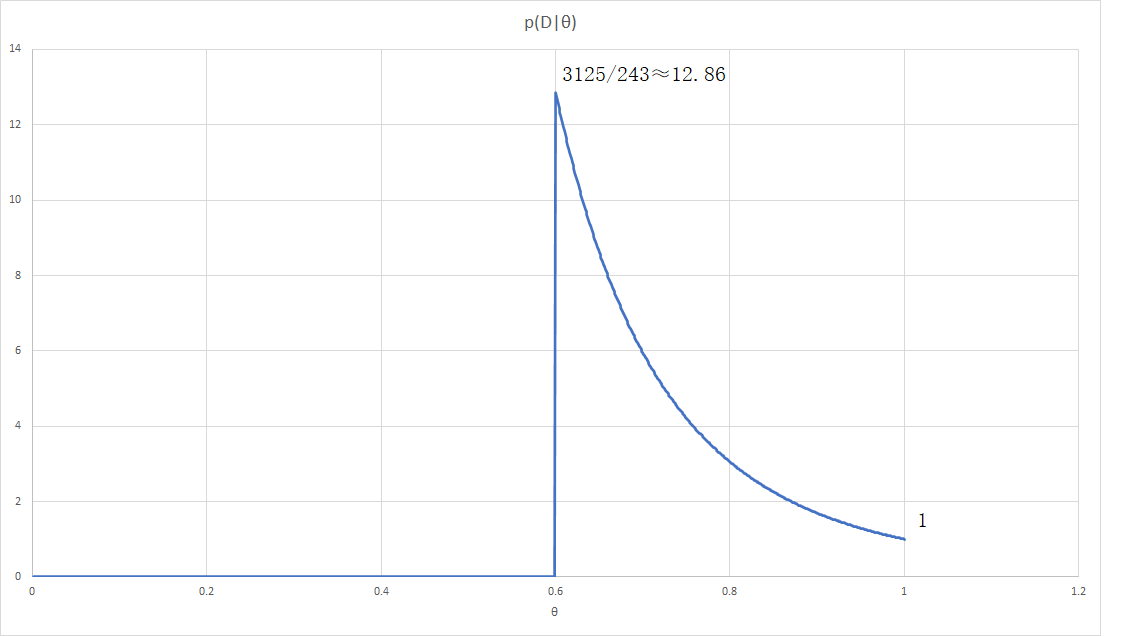
\includegraphics[width=.8\textwidth]{hw2_1.png}            % hw2_1.png是图片文件的相对路径
              \caption{ $p\left(\bm D \mid \theta \right)-\theta$图 }    % caption是图片的标题
              \label{img1}                                               % label标志,方便上下文的引用
          \end{figure}
          $\because p\left(\bm D \mid \theta \right)$ 的值只与 $n ,\theta ,\mathop{max}\limits_{k} x_k = 0.6$ 有关\\
          $\therefore$ 我们不需要知道其他元素值。\\

\end{enumerate}

%%%%%%%%%%%%%%%%%%%%%%%%%%%%%%%%%%%%%%%%%%%%%%%%%%%%%%%%%%%%%%%%%%%%%%%%%%%%%%%%%%%%%%%%%%%%%%%%%

\section*{Queestion 2}
Assume we have training data from a Gaussian distribution of known covariance
$\bm\Sigma$ but unknown mean $\bm\mu$. Suppose further that this mean itself is random, and
characterized by a Gaussian density having mean $\bm m_0$ and covariance $\bm\Sigma_0$ .

\begin{enumerate}
    \item What is the MAP estimator for $\bm\mu$?
    \item Suppose we transform our coordinates by a linear transform $\bm x' = \bm{Ax}$, for nonsingular
          matrix \textbf{A}, and accordingly for other terms. Determine whether your MAP estimator
          gives the appropriate estimate for the transformed mean $\bm\mu'$. Explain.
\end{enumerate}

\section*{Answer 2}
解:
\begin{enumerate}
    \item 由题可知:
          $$
              p\left(\bm\mu\right) = \frac{1}{\left(2\pi\right)^\frac{d}{2}|\bm\Sigma_0|^\frac{1}{2}}
              exp[-\frac{1}{2}\left(\bm\mu-\bm m_0\right)^t\bm\Sigma_0^{-1}\left(\bm\mu-\bm m_0\right)]
          $$
          $$
              \begin{aligned}
                  \ln\left[p\left(\bm D \mid \bm\mu\right)\right]
                   & = \ln \prod\limits_{k=1}^n p\left(\bm x_k \mid \bm \mu \right)                              \\
                   & = \sum\limits_{k=1}^n \ln p\left(\bm x_k \mid \bm \mu \right)                               \\
                   & = \sum\limits_{k=1}^n \ln \{ \frac{1}{\left(2\pi\right)^\frac{d}{2}|\bm\Sigma|^\frac{1}{2}}
                  exp[-\frac{1}{2}\left(\bm x_k-\bm\mu\right)^t\bm\Sigma^{-1}\left(\bm x_k-\bm \mu\right)] \}    \\
                   & = -\frac{n}{2}\ln\left[\left(2\pi\right)^d|\Sigma|\right]-\sum\limits_{k=1}^n \left[
                      \frac{1}{2}\left(\bm x_k-\bm\mu\right)^t\bm\Sigma^{-1}\left(\bm x_k-\bm \mu\right)\right]
              \end{aligned}
          $$
          $\therefore$均值$\bm\mu$的MAP估计是
          $$
              \begin{aligned}
                  \hat{\bm\mu} & = \mathop{arg} \mathop{max}\limits_{\bm\mu} \{\ln\left[p\left(\bm D
                  \mid \bm\mu\right)\right]\times p\left(\bm\mu\right)\}                                            \\
                               & = \mathop{arg} \mathop{max}\limits_{\bm\mu} \left\{\left[-\frac{n}{2}\ln
                  \left[\left(2\pi\right)^d|\bm\Sigma|\right]-\sum\limits_{k=1}^n \left[\frac{1}{2}\right.
                  \left(\bm x_k-\bm\mu\right)^t\bm\Sigma^{-1}\left(\bm x_k-\bm \mu\right)\right]\right.             \\
                               & \left.\times\left[\frac{1}{\left(2\pi\right)^\frac{d}{2}|\bm\Sigma_0|^\frac{1}{2}}
                      exp[-\frac{1}{2}\left(\bm\mu-\bm m_0\right)^t\bm\Sigma_0^{-1}\left(\bm\mu-\bm m_0\right)]
                      \right]\right\}
              \end{aligned}
          $$
    \item 经过线性变换$\bm x' = \bm{Ax}$之后,训练样本的均值和协方差矩阵变为$\bm\mu, \bm\Sigma$:
          $$
              \bm\mu' = \mathcal{E} \left[\bm x'\right] = \mathcal{E} \left[\bm {Ax}\right]
              = \bm A\mathcal{E} \left[\bm x\right] = \bm{A\mu}
          $$
          $$
              \begin{aligned}
                  \bm\Sigma' & = \mathcal{E} \left[\left(\bm x'-\bm \mu'\right)\left(\bm x'-\bm\mu'
                  \right)^t\right]                                                                     \\
                             & = \mathcal{E} \left[\left(\bm {Ax} -\bm {A\mu} \right)
                  \left(\bm {Ax} -\bm{A\mu} \right)^t\right]                                           \\
                             & = \mathcal{E} \left[\bm A\left(\bm x -\bm\mu \right)\left(\bm x -\bm\mu
                  \right)^t\bm A^t\right]                                                              \\
                             & = \bm {A\Sigma A^t}
              \end{aligned}
          $$
          转换后的均值依然为高斯分布:
          $$
              \begin{aligned}
                  p\left(\bm\mu'\right) & = \frac{1}{\left(2\pi\right)^\frac{d}{2}|\bm\Sigma'_0|^\frac{1}{2}}
                  exp[-\frac{1}{2}\left(\bm\mu'-\bm m'_0\right)^t\bm\Sigma_0^{'-1}\left(\bm\mu'-\bm m'_0\right)] \\
                                        & = \frac{1}{\left(2\pi\right)^\frac{d}{2}|\bm\Sigma'_0|^\frac{1}{2}}
                  exp[-\frac{1}{2}\left(\bm\mu-\bm m_0\right)^t\bm A^t\left(\bm A\bm\Sigma_0\bm A^t\right)^{-1}
                  \bm A\left(\bm\mu-\bm m_0\right)]                                                              \\
                                        & = \frac{1}{\left(2\pi\right)^\frac{d}{2}|\bm\Sigma'_0|^\frac{1}{2}}
                  exp[-\frac{1}{2}\left(\bm\mu-\bm m_0\right)^t\bm A^t\bm \left(\bm A^t\right)^{-1}
                  \left(\bm\Sigma_0\right)^{-1}\left(\bm A\right)^{-1}\bm A\left(\bm\mu-\bm m_0\right)]          \\
                                        & = \frac{1}{\left(2\pi\right)^\frac{d}{2}|\bm A\bm\Sigma_0
                      \bm A^t|^\frac{1}{2}}exp[-\frac{1}{2}\left(\bm\mu-\bm m_0\right)^t\bm
                  \left(\bm\Sigma_0\right)^{-1}\left(\bm\mu-\bm m_0\right)]                                      \\
              \end{aligned}
          $$
          log-likelihood:
          $$
              \begin{aligned}
                  \begin{aligned}
                      \ln\left[p\left(\bm D' \mid \bm\mu'\right)\right]
                       & = \ln \prod\limits_{k=1}^np\left(\bm x'_k \mid \bm \mu' \right)                    \\
                       & = \sum\limits_{k=1}^n \ln p\left(\bm x'_k \mid \bm \mu' \right)                    \\
                       & = \sum\limits_{k=1}^n \ln \{ \frac{1}{\left(2\pi\right)^\frac{d}{2}|\bm\Sigma'|^
                          \frac{1}{2}}exp[-\frac{1}{2}\left(\bm x'_k-\bm\mu'\right)^t\bm\Sigma^{'-1}
                      \left(\bm x'_k-\bm \mu'\right)] \}                                                    \\
                       & = -\frac{n}{2}\ln \left[\left(2\pi\right)^d|\bm\Sigma'|\right]-\sum\limits_{k=1}^n
                      \left[\frac{1}{2}\left(\bm x_k-\bm\mu\right)^t\bm A^t\left(\bm A\bm\Sigma\bm A^t
                      \right)^{-1}\bm A\left(\bm x_k-\bm \mu\right)\right]                                  \\
                       & = -\frac{n}{2}\ln \left[\left(2\pi\right)^d|\bm A\bm\Sigma\bm A^t|\right]
                      -\sum\limits_{k=1}^n \left[\frac{1}{2}\left(\bm x_k-\bm\mu\right)^t\bm A^t\bm
                          \left(\bm A^t\right)^{-1}\left(\bm\Sigma\right)^{-1}\left(\bm A\right)^{-1}
                      \bm A\left(\bm x_k-\bm \mu\right)\right]                                              \\
                       & = -\frac{n}{2}\ln \left[\left(2\pi\right)^d|\bm A\bm\Sigma\bm A^t|\right]
                      -\sum\limits_{k=1}^n \left[\frac{1}{2}\left(\bm x_k-\bm\mu\right)^t\bm
                          \Sigma^{-1}\left(\bm x_k-\bm \mu\right)\right]
                  \end{aligned}
              \end{aligned}
          $$
          最新的对$\bm\mu'$的MAP估计如下:
          $$
              \begin{aligned}
                  \hat{\bm\mu'}
                   & = \mathop{arg} \mathop{max}\limits_{\bm\mu} \{\ln\left[p\left(\bm D \mid \bm\mu\right)\right]
                  \times p\left(\bm\mu\right)\}                                                                    \\
                   & = \mathop{arg} \mathop{max}\limits_{\bm\mu} \left\{\left[-\frac{n}{2}\ln \left[\left(2\pi
                          \right)^d|\bm A\bm\Sigma\bm A^t|\right]-\sum\limits_{k=1}^n \left[\frac{1}{2}
                  \left(\bm x_k-\bm\mu\right)^t\bm\Sigma^{-1}\left(\bm x_k-\bm \mu\right)\right]\right]\right.     \\
                   & \left.\times\left[\frac{1}{\left(2\pi\right)^\frac{d}{2}|\bm A\bm\Sigma_0\bm A^t|^
                      \frac{1}{2}}exp[-\frac{1}{2}\left(\bm\mu-\bm m_0\right)^t\bm\Sigma_0^{-1}\left(\bm\mu-
                  \bm m_0\right)]\right]\right\}
              \end{aligned}
          $$
          通过比较$\hat{\bm\mu}$与$\hat{\bm\mu'}$,可见两者表达式相同,故可用MAP适当估计$\hat{\bm\mu'}$。
\end{enumerate}

%%%%%%%%%%%%%%%%%%%%%%%%%%%%%%%%%%%%%%%%%%%%%%%%%%%%%%%%%%%%%%%%%%%%%%%%%%%%%%%%%%%%%%%%%%%%%%%%%

\section*{Queestion 3}
Consider data $\bm D =  \left \{ \begin{pmatrix} 1\\1 \end{pmatrix},\begin{pmatrix} 3\\3 \end{pmatrix},
    \begin{pmatrix} 2\\\star \end{pmatrix} \right \} $, sampled from a two-dimensional (separable) distribution
$p(x_1,x_2) = p(x_1)p(x_2)$, with (1). As usual, $\ast$ represents a missing feature value.
$$
    p \left(x_1\right) \sim
    \begin{cases}
        \frac{1}{\theta_1}e^{-x_1/\theta_1}, & \mbox{if }x_1\ge 0 \\
        0,                                   & \mbox{otherwise}
    \end{cases}
    \quad and\quad
    p \left(x_2\right) \sim
    \begin{cases}
        \frac{1}{\theta_1}, & \mbox{if }0\leq x_2\leq\theta \\
        0,                  & \mbox{otherwise}
    \end{cases}
    \quad \left(1\right)
$$
\begin{enumerate}
    \item Start with an initial estimate $\theta^0 = \begin{pmatrix} 2\\4 \end{pmatrix}$
          and analytically calculate $𝑄(\theta,\theta^0)$— the E step
          in the EM algorithm. Be sure to consider the normalization of your distribution.
    \item Find the $\theta$ that maximizes your $𝑄(\theta,\theta^0)$ — the M step.
\end{enumerate}

\section*{Answer 3}
解:
$$
    \begin{aligned}
        Q\left(\theta;\theta^0\right)
         & = \mathcal{E}_{x_{32}}\left[\ln p\left(x_g,x_b;\theta\right)\mid\theta^0,D_g\right]               \\
         & = \int_{-\infty}^{+\infty}\left[\ln p\left(x_1\mid\theta\right)+\ln p\left(x_2\mid
        \theta\right)+\ln p\left(x_3\mid\theta\right)\right]p\left(x_{32}\mid\theta^0,x_{31}=2\right)dx_{32} \\
         & = \ln p\left(x_1\mid\theta\right)+\ln p\left(x_2\mid\theta\right)+\int_{-\infty}^{+\infty}
        p\left(x_3\mid\theta\right)p\left(x_{32}\mid\theta^0,x_{31}=2\right)dx_{32}                          \\
         & = \ln p\left(x_1\mid\theta\right)+\ln p\left(x_2\mid\theta\right)+\int_{-\infty}^{+\infty}
        p\left(x_3\mid\theta\right)\frac{p\left(\begin{pmatrix} 2\\x_{32} \end{pmatrix}\mid\theta^0\right)}
        {\underbrace{\int_{-\infty}^{+\infty}p\left(\begin{pmatrix} 2\\x'_{32} \end{pmatrix}
        \mid\theta^0\right)dx'_{32}}_{=1/\left(2e\right)}}dx_{32}                                            \\
         & = \ln p\left(x_1\mid\theta\right)+\ln p\left(x_2\mid\theta\right)+2e\int_{-\infty}^{+\infty}
        \ln\left(\frac{1}{\theta_1}e^{-\frac{2}{\theta_1}}\cdot\frac{1}{\theta_2}\right)\cdot
        \left(\frac{1}{2e}\frac{1}{4}\right)dx_{32}                                                          \\
         & = \ln\left(\frac{1}{\theta_1}e^{-\frac{1}{\theta_1}}\cdot\frac{1}{\theta_2}\right)+
        \ln\left(\frac{1}{\theta_1}e^{-\frac{3}{\theta_1}}\cdot\frac{1}{\theta_2}\right)+
        \frac{1}{4}\ln\left(\frac{1}{\theta_1}e^{-\frac{2}{\theta_1}}\cdot\frac{1}{\theta_2}\right)
        \int_{-\infty}^{+\infty}1dx_{32}                                                                     \\
         & = -2\ln\theta_1\theta_2-\frac{4}{\theta_1}\underbrace{-\frac{1}{4}\left(\ln\theta_1
        \theta_2+\frac{2}{\theta_2}\right)\int_{-\infty}^{+\infty}1dx_{32}}_{\equiv K}
    \end{aligned}
$$
Case 1: $3\leq\theta_2\leq4$,
$$
    \begin{aligned}
        Q\left(\theta;\theta^0\right)
         & = -2\ln\theta_1\theta_2-\frac{4}{\theta_1}-\frac{1}{4}\left(\ln\theta_1\theta_2+\frac{2}
        {\theta_2}\right)\int_{0}^{\theta_2}1dx_{32}                                                       \\
         & = -2\ln\theta_1\theta_2-\frac{4}{\theta_1}-\frac{\theta_2}{4}\left(\ln\theta_1\theta_2+\frac{2}
        {\theta_2}\right)
    \end{aligned}
$$
$$
    \begin{aligned}
        \frac{\partial Q}{\partial \theta_1}
         & = -2/\theta_1+4/\left(\theta_1^2\right)-\theta_2/\left(4\theta_1\right)+
        \theta_2/\left(2\theta_1^2\right)                                                            \\
         & = \frac{\left(-8\theta_1+16\right)+\left(-\theta_1\theta_2+2\theta_2\right)}{4\theta_1^2} \\
         & = \frac{8\left(2-\theta_1\right)+\theta_2\left(2-\theta_1\right)}{4\theta_1^2}            \\
         & = \frac{\left(8+\theta_2\right)\left(2-\theta_1\right)}{4\theta_1^2}
    \end{aligned}
$$
令$\frac{\partial Q}{\partial \theta_1} = 0$,则$\theta_1=2$或$\theta_2=-8$,而
$
    p \left(x_2\right) \sim
    \begin{cases}
        \frac{1}{\theta_1}, & \mbox{if }0\leq x_2\leq\theta \\
        0,                  & \mbox{otherwise}
    \end{cases}
$
$\therefore \theta_1=2 \\
    Q = -2\ln 2\theta_2-2-\frac{\theta_2}{4}\left(\ln 2\theta_2+1\right)
    = -\ln 2\theta_2\left(2+\frac{\theta_2}{4}\right)-\left(2+\frac{\theta_2}{4}\right)
    = -\left(2+\frac{\theta_2}{4}\right)\left(1+\ln 2\theta_2\right)
$ \\
可见,$\theta_2$越大,Q越小,又 $3\leq\theta_2\leq4$,$\therefore$ 当$\theta_2=3$,有$Q_{max} \approx -7.677$。\\
Case 2: $\theta_2\geq 4$,
$$
    \begin{aligned}
        Q\left(\theta;\theta^0\right)
         & = -2\ln\theta_1\theta_2-\frac{4}{\theta_1}-\frac{1}{4}\left(\ln\theta_1\theta_2+\frac{2}
        {\theta_2}\right)\int_{0}^{4}1dx_{32}                                                       \\
         & = -2\ln\theta_1\theta_2-\frac{4}{\theta_1}-\left(\ln\theta_1\theta_2+\frac{2}
        {\theta_2}\right)                                                                           \\
         & = -3\ln\theta_1\theta_2-\frac{6}{\theta_1}
    \end{aligned}
$$
$$
    \begin{aligned}
        \frac{\partial Q}{\partial \theta_1}
         & = -3/\theta_1+6/\left(\theta_1^2\right) \\
         & = \frac{6-3\theta_1}{\theta_1^2}
    \end{aligned}
$$
令$\frac{\partial Q}{\partial \theta_1} = 0$,则$\theta_1=2$,\\
$Q = -3\ln 2\theta_2-3$\\
可见,$\theta_2$越大,Q越小,当$\theta_2=4$,有$Q_{max} \approx -9.238$。\\
Case 3: $\theta_2=otherwise$, K=0。\\
综上,
$$
    Q_{max} = \begin{cases}
        -7.677, & \mbox{if }3\leq \theta_2\leq 4, \bm \theta = \left[ \begin{matrix}2\\3\end{matrix}\right] \\
        -9.238, & \mbox{if } \theta_2\geq 4, \bm \theta = \left[ \begin{matrix}2\\4\end{matrix}\right]
    \end{cases}
$$

%%%%%%%%%%%%%%%%%%%%%%%%%%%%%%%%%%%%%%%%%%%%%%%%%%%%%%%%%%%%%%%%%%%%%%%%%%%%%%%%%%%%%%%%%%%%%%%%%

\section*{Queestion 4}
Consider training an HMM by the Forward-backward algorithm, for a single
squence of length T where each symbol could be one of c values. What is the
computational complexity of a single revision of all values $\hat{a}_{ij}$
and $\hat{b}_{jk}$?

\section*{Answer 4}

解:\\
我们定义从状态$\omega_i\left(t-1\right)$转移到$\omega_j\left(t\right)$的概率$\gamma_{ij}\left(t\right)$,\\
$$
    \gamma_{ij}\left(t\right) = \frac{\alpha_i\left(t-1\right)a_{ij}b_{jk}\beta_j\left(t\right)}{P
    \left(\bm V^T\mid\bm\theta\right)}
$$
其中,$P\left(\bm V^T\mid\bm\theta\right)$是模型用任意的隐状态路径产生序列$\bm V^T$的概率。
这样$\gamma_{ij}\left(t\right)$就是在产生序列的条件下从状态$\omega_i\left(t-1\right)$转移到
$\omega_j\left(t\right)$的概率。\\
序列从状态$\omega_i\left(t-1\right)$转移到$\omega_j\left(t\right)$的预期值是
$\sum_{t=1}^T\gamma_{ij}\left(t\right)$,而从$\omega_i$的任何转移的总预期数为
$\sum_{t=1}^T\sum_k\gamma_{ik}\left(t\right)$,这样,隐状态转移概率$\hat a_{ij}$和
发出显状态概率$\hat b_{jk}$可如此求出:\\
$$
    \begin{aligned}
        \hat a_{ij} = \frac{\sum_{t=1}^T\gamma_{ij}\left(t\right)}
        {\sum_{t=1}^T\sum_k\gamma_{ik}\left(t\right)} \\
        \hat b_{jk} = \frac{\mathop{\sum_{t=1}^T}\limits_{v\left(t\right)=v_k}\sum_l\gamma_{jl}\left(t\right)}
        {\sum_{t=1}^T\sum_l\gamma_{jl}\left(t\right)}
    \end{aligned}
$$
可见,$\hat{a}_{ij}$和$\hat{b}_{jk}$复杂度都为$O\left(c^2T\right)$

%%%%%%%%%%%%%%%%%%%%%%%%%%%%%%%%%%%%%%%%%%%%%%%%%%%%%%%%%%%%%%%%%%%%%%%%%%%%%%%%%%%%%%%%%%%%%%%%%

\section*{Queestion 5}
Consider a normal $p\left(x\right)\sim N\left(\mu,\sigma^2\right)$ and Parzen-window function
$\phi\left(x\right)\sim N\left(0, 1\right)$ . Show that the Parzen-window estimate
$$
    p_n\left(x\right) = \frac{1}{nh_n}\sum\limits_{i=1}^n\phi\left(\frac{x-x_i}{h_n}\right)
$$
has the following properties: \\
1. $\bar p_n\left(x\right)\sim N\left(\mu,\sigma^2+h_n^2\right)$\\
2. $Var\left[p_n\left(x\right)\right] \approx \frac{1}{2nh_n\sqrt\pi}p\left(x\right)$

\section*{Answer 5}
解:由题可知
$$
    \begin{aligned}
         & p\left(x\right) = \frac{1}{\sqrt{2\pi}\sigma}exp\left[-\frac{1}{2}\left(\frac{x-\mu}{\sigma}\right)^2\right] \\
         & \phi\left(x\right) = \frac{1}{\sqrt{2\pi}}exp\left[-\frac{x^2}{2}\right]                                     \\
         & p_n\left(x\right) = \frac{1}{nh_n}\sum\limits_{i=1}^n\phi\left(\frac{x-x_i}{h_n}\right)
    \end{aligned}
$$
\begin{enumerate}
    \item
          $$
              \begin{aligned}
                  \bar p_n\left(x\right) & = \mathcal{E}\left[p_n\left(x\right)\right]                      \\
                                         & = \frac{1}{nh_n}\sum\limits_{i=1}^n\mathcal{E}
                  \left[\phi\left(\frac{x-x_i}{h_n}\right)\right]                                           \\
                                         & = \frac{1}{h_n}\int_{-\infty}^{+\infty}\phi\left(
                  \frac{x-v}{h_n}\right)p\left(v\right)dv                                                   \\
                                         & = \frac{1}{h_n}\int_{-\infty}^{+\infty} \frac{1}{
                      \sqrt{2\pi}}exp\left[-\frac{1}{2}\left(\frac{x-v}{h_n}\right)^2\right]\frac{1}
                  {\sqrt{2\pi}\sigma}exp\left[-\frac{1}{2}\left(\frac{x-\mu}{\sigma}\right)^2\right]dv--(1) \\
                                         & = \frac{1}{2\pi h_n\sigma}\int_{-\infty}^{+\infty}exp
                  \left[-\frac{1}{2}\left(\frac{x^2}{h_n^2}+\frac{\mu^2}{\sigma^2}\right)
                      -\frac{1}{2}v^2\underbrace{\left(\frac{1}{h_n^2}+\frac{1}{\sigma^2}\right)}
                      _{\equiv 1/\theta^2}+v\underbrace{\left(\frac{x}{h_n^2}+\frac{\mu}{\sigma}
                          \right)}_{\equiv \alpha/\theta^2}\right]dv
              \end{aligned}
          $$
          即令
          $$
              \begin{cases}
                  \theta^2 = \frac{1}{1/h_n^2+1/\sigma^2} = \frac{h_n^2\sigma^2}{h_n^2+\sigma^2} \\
                  \alpha = \theta^2\left(\frac{x}{h_n^2}+\frac{\mu}{\sigma^2}\right)
              \end{cases}
          $$
          $$
              \begin{aligned}
                  \bar p_n\left(x\right) & = \frac{1}{2\pi h_n\sigma}exp\left[-\frac{1}{2}
                      \left(\frac{x^2}{h_n^2}+\frac{\mu^2}{\sigma^2}\right)\right]\int_{-\infty}^{+\infty}
                  exp\left[-\frac{1}{2}\left(\frac{v^2}{\theta^2}-\frac{2v\alpha}{\theta^2}
                  +\frac{\alpha^2}{\theta^2}-\frac{\alpha^2}{\theta^2}\right)\right]dv                       \\
                                         & = \frac{1}{2\pi h_n\sigma}exp\left[-\frac{1}{2}
                      \left(\frac{x^2}{h_n^2}+\frac{\mu^2}{\sigma^2}-\frac{\alpha^2}{\theta^2}
                      \right)\right]\int_{-\infty}^{+\infty}exp\left[-\frac{1}{2}
                  \left(\frac{v-\alpha}{\theta}\right)^2\right]dv                                            \\
                                         & = \frac{1}{2\pi h_n\sigma}exp\left[-\frac{1}{2}
                      \left(\frac{x^2}{h_n^2}+\frac{\mu^2}{\sigma^2}-\frac{\alpha^2}{\theta^2}
                      \right)\right]\int_{-\infty}^{+\infty}exp\left[-\left(\frac{w}{\sqrt{2}\theta}\right)^2
                  \right]dw                                                                                  \\
                                         & = \frac{1}{2\pi h_n\sigma}exp\left[-\frac{1}{2}
                      \left(\frac{x^2}{h_n^2}+\frac{\mu^2}{\sigma^2}-\frac{\alpha^2}{\theta^2}
                  \right)\right]\sqrt{\pi}\sqrt{2}\theta                                                     \\
                                         & = \frac{\theta}{\sqrt{2\pi} h_n\sigma}exp\left[-\frac{1}{2}
                      \left(\frac{x^2}{h_n^2}+\frac{\mu^2}{\sigma^2}-\frac{h_n^2\sigma^2}{h_n^2+\sigma^2}
                  \left(\frac{x}{h_n^2}+\frac{\mu}{\sigma^2}\right)^2\right)\right]                          \\
                                         & = \frac{1}{\sqrt{2\pi}\sqrt{h_n^2+\sigma^2}}exp\left[-\frac{1}{2}
                      \frac{\left(x-\mu\right)^2}{h_n^2+\sigma^2}\right]--(2)
              \end{aligned}
          $$
          由此可见,$\bar p_n\left(x\right)\sim N\left(\mu,\sigma^2+h_n^2\right)$ 。
    \item
          $$
              \begin{aligned}
                  Var\left[p_n\left(x\right)\right]
                   & = Var\left[\frac{1}{nh_n}\sum\limits_{i=1}^n
                  \left[\phi\left(\frac{x-x_i}{h_n}\right)\right] \right] \\
                   & = \frac{1}{n^2h_n^2}\sum\limits_{i=1}^n
                  Var\left[\phi\left(\frac{x-x_i}{h_n}\right)\right]      \\
                   & = \frac{1}{nh_n^2}
                  Var\left[\phi\left(\frac{x-v}{h_n}\right)\right]        \\
                   & = \frac{1}{nh_n^2}
                  \left\{\mathcal{E}\left[\phi^2\left(\frac{x-v}{h_n}\right)\right]-
                  \left\{\mathcal{E}\left[\phi\left(\frac{x-v}{h_n}\right)\right]\right\}^2\right\}
              \end{aligned}
          $$
          其中
          $$
              \begin{aligned}
                  \mathcal{E}\left[\phi^2\left(\frac{x-v}{h_n}\right)\right]
                   & = \int \phi^2\left(\frac{x-v}{h_n}\right)p\left(v\right)dv      \\
                   & = \int_{-infty}^{+infty}\frac{1}{2\pi}
                  exp\left[-\frac{1}{2}\left(\frac{x-v}{h_n}\right)^22\right]\frac{1}{\sqrt{2\pi}\sigma}
                  exp\left[-\frac{1}{2}\left(\frac{x-\mu}{\sigma}\right)^2\right]dv  \\
                   & \overset{h_n/\sqrt{2}->h_n}{=} \frac{h_n/\sqrt{2}}{\sqrt{2\pi}}
                  \frac{1}{h_n/\sqrt{2}}\int_{-\infty}^{+\infty} \frac{1}{
                      \sqrt{2\pi}}exp\left[-\frac{1}{2}\left(\frac{x-v}{h_n/\sqrt{2}}\right)^2\right]\frac{1}
                  {\sqrt{2\pi}\sigma}exp\left[-\frac{1}{2}\left(\frac{x-\mu}{\sigma}\right)^2\right]dv
              \end{aligned}
          $$
          根据式子(1)和(2),我们可以得到:
          $$
              \begin{aligned}
                  \mathcal{E}\left[\phi^2\left(\frac{x-v}{h_n}\right)\right]
                   & = \frac{h_n/\sqrt{2}}{\sqrt{2\pi}} \frac{1}{\sqrt{2\pi}
                      \sqrt{h_n^2/2+\sigma^2}}exp\left[-\frac{1}{2}\cdot
                  \frac{\left(x-\mu\right)^2}{h_n^2/2+\sigma^2}\right]       \\
                   & = \frac{h_n}{2\sqrt{\pi}}\frac{1}{\sqrt{2\pi}
                      \sqrt{h_n^2/2+\sigma^2}}exp\left[-\frac{1}{2}\cdot
                      \frac{\left(x-\mu\right)^2}{h_n^2/2+\sigma^2}\right]
              \end{aligned}
          $$
          所以可以得到$Var\left[p_n\left(x\right)\right]$的第1项:
          $$
              \begin{aligned}
                  \frac{1}{nh_n^2}\mathcal{E}\left[\phi^2\left(\frac{x-v}{h_n}\right)\right]
                   & = \frac{1}{nh_n^2}\frac{h_n}{2\sqrt{\pi}}\frac{1}{\sqrt{2\pi}
                      \sqrt{h_n^2/2+\sigma^2}}exp\left[-\frac{1}{2}\cdot
                  \frac{\left(x-\mu\right)^2}{h_n^2/2+\sigma^2}\right]                           \\
                   & = \frac{1}{2nh_n\sqrt{\pi}}\frac{1}{\sqrt{2\pi}
                      \sqrt{h_n^2/2+\sigma^2}}exp\left[-\frac{1}{2}\cdot
                  \frac{\left(x-\mu\right)^2}{h_n^2/2+\sigma^2}\right]                           \\
                   & \approx \frac{1}{2nh_n\sqrt{\pi}}\left\{\frac{1}{\sqrt{2\pi}\sigma}
                  exp\left[-\frac{1}{2}\cdot\frac{\left(x-\mu\right)^2}{\sigma^2}\right]\right\} \\
                   & = \frac{1}{2nh_n\sqrt{\pi}}p\left(x\right)
              \end{aligned}
          $$
          上式子$\approx$是因为$\sqrt{h_n^2/2+\sigma^2}\approx\sigma$。\\
          类似地$Var\left[p_n\left(x\right)\right]$的第2项:
          $$
              \begin{aligned}
                  \frac{1}{nh_n^2}\left\{\mathcal{E}\left[\phi\left(\frac{x-v}{h_n}\right)\right]\right\}^2
                   & = \frac{1}{nh_n^2}\left[\int_{-\infty}^{+\infty}\phi\left(\frac{x-v}{h_n}\right)
                  p\left(v\right)dv\right]^2                                                          \\
                   & = \frac{1}{nh_n^2}\left\{ \int_{-\infty}^{+\infty} \frac{1}{\sqrt{2\pi}}
                  exp\left[-\frac{1}{2}\left(\frac{x-v}{h_n}\right)^2\right]\frac{1}{\sqrt{2\pi}\sigma}
                  exp\left[-\frac{1}{2}\left(\frac{x-\mu}{\sigma}\right)^2\right]dv\right\}^2         \\
                   & = \frac{1}{nh_n^2}\left\{ h_n\frac{1}{\sqrt{2\pi}\sqrt{h_n^2+\sigma^2}}
                  exp\left[-\frac{1}{2}\cdot\frac{\left(x-\mu\right)^2}{h_n^2+\sigma^2}\right]
                  \right\}^2                                                                          \\
                   & = \frac{h_n^2}{nh_n^2}\left\{\frac{1}{\sqrt{2\pi}\sqrt{h_n^2+\sigma^2}}
                  exp\left[-\frac{1}{2}\cdot\frac{\left(x-\mu\right)^2}{h_n^2+\sigma^2}\right]
                  \right\}^2                                                                          \\
                   & \approx \frac{1}{n} \left\{\frac{1}{\sqrt{2\pi}\sigma}
                  exp\left[-\frac{1}{2}\cdot\frac{\left(x-\mu\right)^2}{\sigma^2}\right]\right\}^2    \\
                   & = \frac{1}{n}p^2\left(x\right)                                                   \\
                   & \approx 0
              \end{aligned}
          $$
          $\therefore Var\left[p_n\left(x\right)\right] \approx \frac{1}{2nh_n\sqrt\pi}p\left(x\right)$
\end{enumerate}

%%%%%%%%%%%%%%%%%%%%%%%%%%%%%%%%%%%%%%%%%%%%%%%%%%%%%%%%%%%%%%%%%%%%%%%%%%%%%%%%%%%%%%%%%%%%%%%%%

\section*{Queestion 6}
Explore the effect of r on the accuracy of nearest-neighbor search based on par-
tial distance. Assume we have a large number n of points randomly placed in a d-
dimensional hypercube. Suppose we have a test point x, also selected randomly
in the hypercume, and find its nearest neighbor. By definition, if we use the full
d-dimensional Euclidean distance, we are guaranteed to find its nearest neigh-
bor. Suppose though we use the partial distance
$$
    D_r\left(x,x'\right) = \left(\sum\limits_{i=1}^r\left(x_i-x'_i\right)^2\right)^{1/2}
$$
\begin{enumerate}
    \item Plot the probability that a partial distance search finds the true closest neighbor of
          an arbitrary point x as a function of r for fixed $ n \left(1 \leq r \leq d\right)$
          for $d = 10$.
    \item Consider the effect of r on the accuracy of a nearest-neighbor classifier. Assume we
          have n/2 prototypes from each two categories in a hypercube of length 1 on a side.
          The density for each category is separable into the product of (linear) ramp functions,
          highest at one side, and zero at the other side of the range. Thus the density for category
          $\omega_1$  is highest at $\left(0,0,...0\right)^t$  and zero at $\left(1,1,...1\right)^t$,
          while the density for $\omega_2$ is highest at $\left(1,1,...1\right)^t$ and zero at
          $\left(0,0,...0\right)^t$ . State by inspection the Bayesian decision boundary.
\end{enumerate}

\section*{Answer 6}
解:
\begin{enumerate}
    \item
          假设$n$个样本在$d$维相互独立,均匀分布,\\
          则每个维度的样本数为:$n^{1/d}$ \\
          $r$维上的样本数为:$n^{r/d}$ \\
          $\therefore r$维上选中正确数据作为最近邻的概率为:\\
          $$\begin{aligned}p =  n^{r/d}/n = n^{\frac{r}{d}-1}\end{aligned}$$
          $\because d = 10$\\
          $\therefore p = n^{\frac{r}{10}-1}$ \\
          当 $n = 2,3,4,...,10$,$p-r$图如下所示:\\
          \begin{figure}[H]
              \centering
              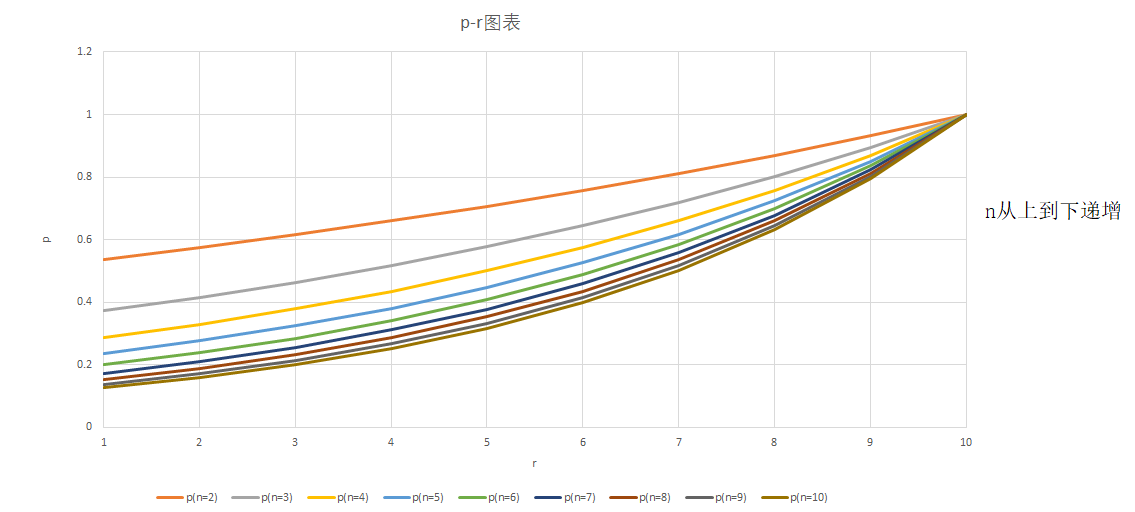
\includegraphics[width=.8\textwidth]{hw2_2.png}
              \caption{ $p-r$图 }
              \label{img2}
          \end{figure}

    \item
          1维:$x_1^*=0.5$ \\
          2维:$x_2^*=1-x_1$ \\
          3维:$x_1x_2x_3 = \left(1-x_1\right)\left(1-x_2\right)\left(1-x_3\right)
              \Rightarrow x_3^* = \frac{\left(1-x_1\right)\left(1-x_2\right)}{1-x_1-x_2+2x_1x_2}$ \\
          ... \\
          d维:$\prod\limits_{i=1}^dx_i = \prod\limits_{i=1}^d\left(1-x_i\right)$
\end{enumerate}

\end{document}